\documentclass[a4j]{jsreport}
\usepackage[dvipdfmx]{graphicx}
\usepackage{multicol}
\usepackage{amsmath}
\graphicspath{{./figure/}}

\begin{document}

% 表紙
\begin{titlepage}
\vspace{5cm}
\centering
{\Huge トルエンの空気酸化による安息香酸の製造}\\
\vspace{2cm}
\centering
{\Large 1講座 移動現象論分野}\\
\vspace{0.5cm}
\centering
{\large 荊尾太雅 , 宮本奏汰}\\
\vspace{3cm}
\begin{table}[htbp]
    \begin{center}
        \begin{tabular}[htbp]{ll}
            \multicolumn{2}{c}{{\LARGE keyword}}\\
            {\Large 空気酸化}&{\Large Air oxidation}\\
            {\Large 気液反応}&{\Large Gas-liquid reaction}\\
            {\Large 晶析}&{\Large Crystallization}\\
            {\Large 多変数同時全体最適化}&{\Large Multi-variable simultaneous optimization}\\
            {\Large }&{\Large air}\\
        \end{tabular}
    \end{center}
\end{table}

\end{titlepage}


\newpage
\pagenumbering{roman}
\setcounter{tocdepth}{2}
\tableofcontents
    
\newpage

% 本文
\pagenumbering{arabic}
\chapter{緒言}
安息香酸は、主としてフェノールの原料となる他、その塩が食品や化粧品などの添加物として広く利用されている。
2014年には世界全体で48万トンが製造されており、新興国での需要から、2024年には生産量が64万トンとなると見込まれている。
そこで、私たちは原料として安価なトルエンを使用し、空気酸化することで安息香酸を製造するプロセスを
題材とし、本プロセス設計演習において検討することにした。

\newpage
\chapter{プロセスの概要}
\section{プロセスの概要}
本設計で対象とするのは、トルエンを空気酸化することにより安息香酸を製造するプロセスである。
プロセス全体の概略図を図\ref{プロセス全体のの概略図}に示す。
\begin{figure}[h]
    \label{プロセス全体のの概略図}
    \begin{center}
        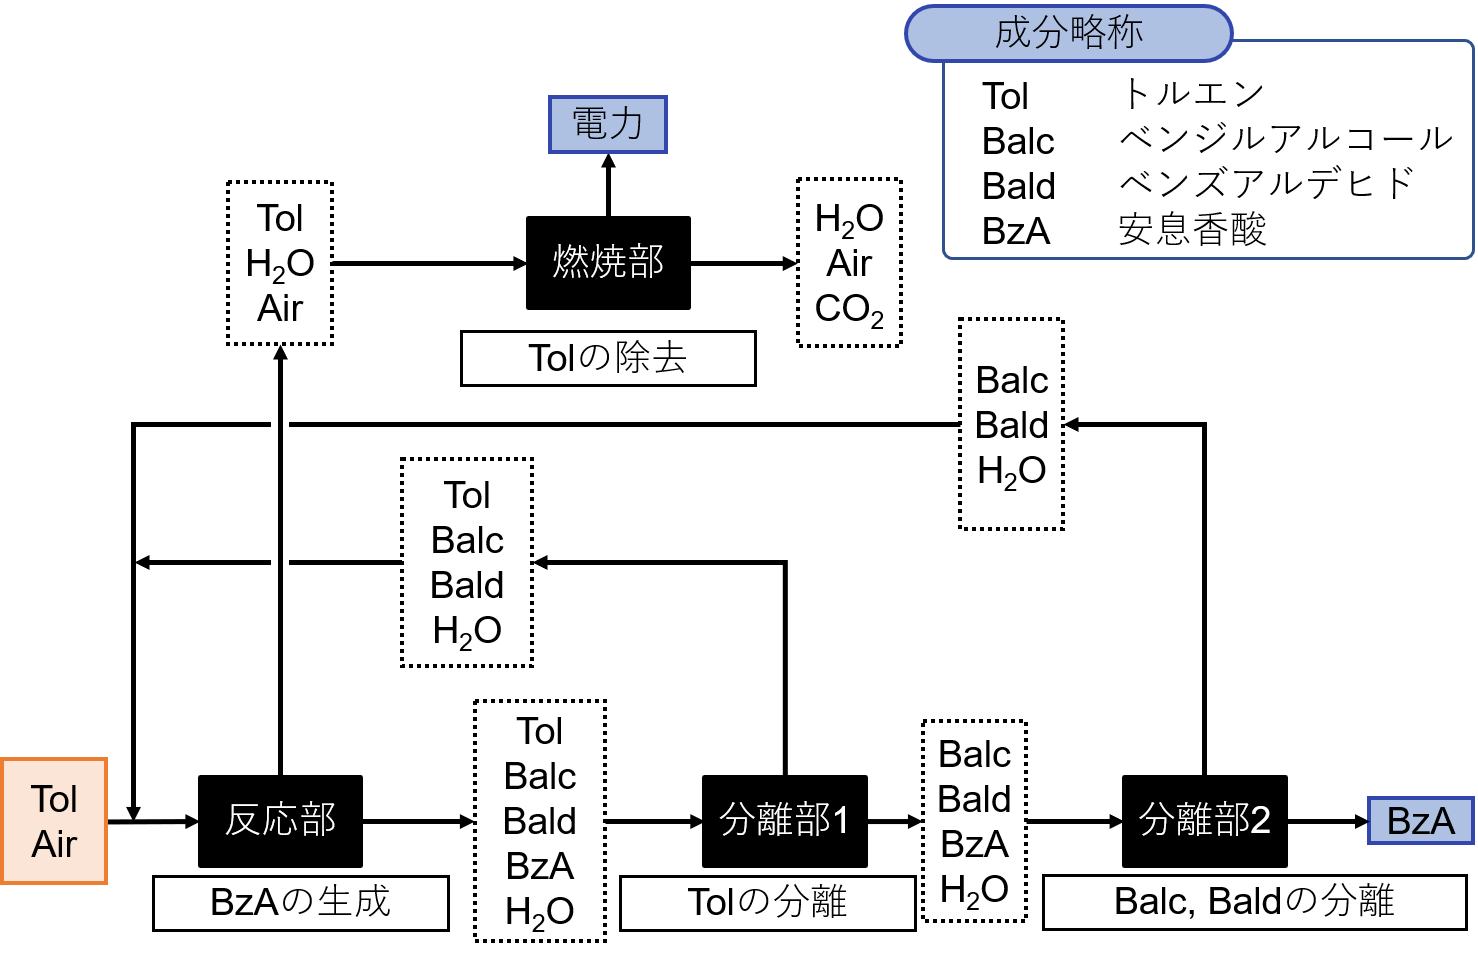
\includegraphics[scale=0.7]{processOutline.png}
        \caption{プロセス全体の概略図}
    \end{center}
\end{figure}

\section{設計条件}
\begin{enumerate}
    \item 生産要求は、99.0wt\%以上の安息香酸を年2万トンとする。\\
    \item 工場の稼働時間は、1日24時間、年300日とする。\\
    \item 原料として、純度100\%のトルエンおよび、組成を窒素79mol\%酸素21mol\%とする空気を用いる。
             ただし、両原料は25℃、1barで供給されるものとする。\\
    \item 減価償却期間は7年である。\\
    \item 圧力損失、熱損失、制御系については考慮しない。
\end{enumerate}
HYSISを用いての物性推算はUNIQUAC式によって行った。

\newpage
\chapter{反応部}

反応部の概略図を図 \ref{反応部設計結果の概略図} に示す。
\begin{figure}[h]
    \label{反応部設計結果の概略図}
    \begin{center}
        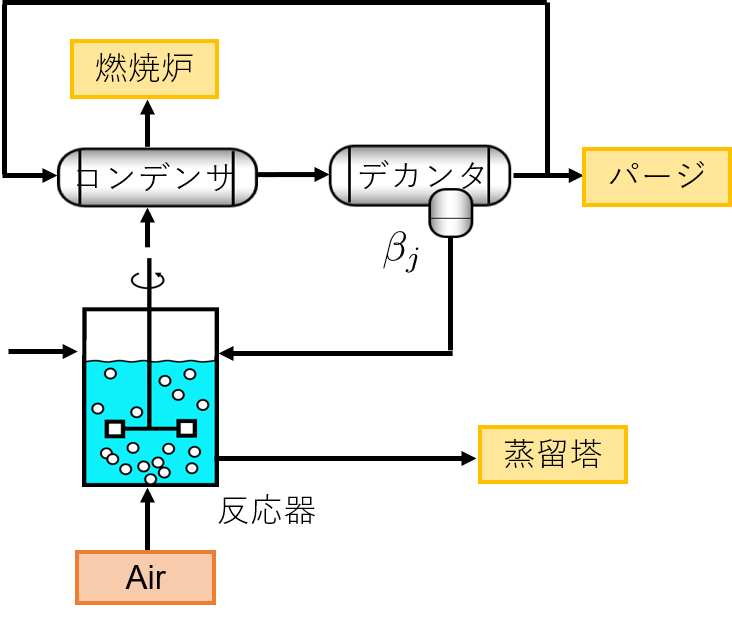
\includegraphics[scale=0.7]{ReactionSection.png}
        \caption{反応部概略図}
    \end{center}
\end{figure}

\section{反応機構}

\section{反応器選定}
流通式の気液反応器の種類には、拡散速度に対して不利な順に、気泡塔、気液攪拌槽、充填塔などがある。
最大反応速度と最大拡散速度の比を表す八田数を事前に概算し、
参考文献\cite{化工便覧}の選定基準に基づき、八田数が0.1より小さいなら気泡塔、
5より大きければ充填塔、中間域ならば気液攪拌槽を選択した。
今回は気液攪拌槽型反応器を選択した。実際のプロセスでは気泡塔も選択される。\\
八田数の定義式
\begin{equation}
    \gamma = \frac{(\text{最大反応速度})}{(\text{最大拡散速度})} = \frac{(C_{\mathrm{ B}}kD_{\mathrm{ B}})^{1/2}}{k_{\mathrm{ L}}}
\end{equation}

\section{設計方程式}
液相は完全混合状態として、気相は鉛直方向に向かう押し出し流れとなっているとして設計を行った。
用いた仮定は以下のようになる。
\begin{itemize} 
    \item[-] 気相は水平方向に一様な濃度分布を持つ。
    \item[-] 気相側境膜抵抗は無視できる
    \item[-] 液相は完全混合状態である。
    \item[-] 窒素、酸素はヘンリー則に従い、その他の物質はラウール則に従う。
\end{itemize}
以上の仮定および、蒸発油分を還流する機構を含めて、設計方程式(\ref{液相物質収支式}),(\ref{気相物質収支式})を立式した。\\
\begin{equation}
    \label{液相物質収支式}
    0=F^{\mathrm{ in}}_{\mathrm{ liq},j}-F^{\mathrm{ out}}_{\mathrm{ liq},j} -(1-\beta_j) k_{\mathrm{ L}}a
    \int^{V_{\mathrm{ tot}}}_0(C_j - C^{\mathrm{ sat}}_j)\mathrm{ d}V + r_j V_{\mathrm{ L}}
\end{equation}
\begin{equation}
    \label{気相物質収支式}                                                
    \frac{\mathrm{ d}F_{\mathrm{ gas},j}}{\mathrm{ d}V} = k_{\mathrm{ L}}a(C_j - C^{\mathrm{ sat}}_j)
\end{equation}

\section{物質移動容量係数の推算}
物質移動容量係数の推算に用いた各相関式を記す。

液相側物質移動係数の相関式\\
小気泡の場合
\begin{equation}
    k_{\mathrm{ L}} = 0.31Sc_{\mathrm{ L}}^{-2/3}(g \Delta \rho \mu_{\mathrm{ L}}/\rho_{\mathrm{ L}}^2)^{1/3}
\end{equation}
大気泡の場合
\begin{equation}
    k_{\mathrm{ L}} = 0.42Sc_{\mathrm{ L}}^{-1/2}(g \Delta \rho \mu_{\mathrm{ L}}/\rho_{\mathrm{ L}}^2)^{1/3}
\end{equation}
比表面積の相関式
\begin{equation}
    a = 1.44(\frac{P_{\mathrm{ V}}^{0.4} \rho_{\mathrm{ L}}^{0.2} }{ \sigma^{0.6}})(\frac{u_{\mathrm{ G}}}{u_{\mathrm{ t}}})^{0.5}(\frac{P_{\mathrm{ T}}}{P_{\mathrm{ G}}})(\frac{\rho_{\mathrm{ G}}}{\rho_{\mathrm{ a}}})^{0.16}
\end{equation}

上記の2式を利用するために用いた相関式を以下に記す。

ガスホールドアップの相関式
\begin{equation}
    \varepsilon_{\mathrm{ G}} = (\frac{u_{\mathrm{ G}}\varepsilon_{\mathrm{ G}}}{u_{\mathrm{ t}}}) ^{0.5} + 0.000216 \times(\frac{P_{\mathrm{ V}}^{0.4} \rho_{\mathrm{ L}}^{0.2} }{ \sigma^{0.6}})(\frac{u_{\mathrm{ G}}}{u_{\mathrm{ t}}})^{0.5}(\frac{P_{\mathrm{ T}}}{P_{\mathrm{ G}}})(\frac{\rho_{\mathrm{ a}}}{\rho_{\mathrm{ G}}})^{0.16}
\end{equation}
気泡の体積平均径の相関式
\begin{equation}
    d_{\mathrm{ vs}} = 4.15 (\frac{\sigma^{0.6}}{P_{\mathrm{ V}}^{0.4} \rho_{\mathrm{ L}}^{0.2}})(\frac{P_{\mathrm{ G}}}{P_{\mathrm{ T}}})(\frac{\rho_{\mathrm{ a}}}{\rho_{\mathrm{ G}}})^{0.16} \varepsilon_{\mathrm{ G}}^{0.5} + 0.0009
\end{equation}
気泡の終末速度の相関式
\begin{equation}
    u_{\mathrm{ t}} = (\frac{4\Delta \rho g d_{\mathrm{ vs}}}{3C_{\mathrm{ D}}\rho_{\mathrm{ L}}})^{0.5}
\end{equation}

さらに、上記の相関式を利用するために用いた物性値の推算式、および変数の定義式などの諸式を以下に記す。

抗力係数の相関式
\begin{equation}
    C_{\mathrm{ D}} = \mathrm{ max}[\frac{24}{Re}(1+0.15Re^{0.687}), \frac{8}{3}\frac{Eo}{Eo+4}]
\end{equation}
拡散係数の推算\\
wilke-changの式
\begin{equation}
    D_{12} = \frac{2.946\times 10^{-11}(\beta M_{\mathrm{ r,2}})^{1/2} T} {\mu_2 V_{\mathrm{ b,1}}^{0.6}}
\end{equation}
Einstin-Stokesの式
\begin{equation}
    \frac{D \mu}{T} = \mathrm{ const}
\end{equation}

界面張力の推算\\
界面張力の温度依存性に関する相関式
\begin{equation}
    \sigma \propto \{1-(T/T_{\mathrm{ c}}) \}^n    
\end{equation}

気泡レイノルズ数の定義式
\begin{equation}
    Re = \frac{\rho_{\mathrm{ L}}u_{\mathrm{ t}}d_{\mathrm{ vs}}}{\mu_{\mathrm{ L}}}
\end{equation}
エトベス数の定義式
\begin{equation}
    Eo = \frac{g \Delta \rho d_{\mathrm{ vs}}^2}{\sigma}
\end{equation}
以上の式を用いる際にデータとして、\\
参考文献[]からトルエンの界面張力\,$\sigma\,=\,0.81\,\mathrm{ N\,m^{-2}}$とした。

\section{反応器設計結果} 
最終結果における反応器の詳細を表\ref{反応器設計結果の表}に示す。
\begin{table}[h]
    \label{反応器設計結果の表}
    \caption{反応器設計結果}
    \begin{center}
        \begin{tabular}{lc}\hline
            \multicolumn{1}{c}{項目}       &  値    \\   \hline
            反応器内圧力\,[bar]             &7.00   \\
            反応器内温度\,[$^\circ$C]       &170    \\
            反応器体積\,[m$^3$]             &14.6    \\
            気液総体積\,[m$^3$]             &8.25   \\
            ガスホールドアップ\,[\,-\,]     &0.115  \\
            液平均滞留時間\,[h]             &0.478  \\
            物質移動容量係数\,[s$^{-1}$]    &0.470  \\
            液相物質移動係数\,[m s$^{-1}$]  &0.00172 \\
            比界面積\,[m$^{-1}$]            &273    \\
            反応器空間率\,[\,-\,]           &0.435  \\
            総攪拌動力\,[kW]                &8.25   \\
            気泡体積平均径\,[\,mm\,]        &2.53    \\
            エトベス数\,[\,-\,]            &1480     \\
            気泡レイノルズ数\,[\,-\,]       &1170    \\\hline
        \end{tabular}
    \end{center}
\end{table}

\section{反応部設計結果}
最適化後の最終結果における反応部の物質収支を図\ref{反応部設計結果の図}中に示す。
\begin{figure}[h]
    \label{反応部設計結果の図}
    \begin{center}
        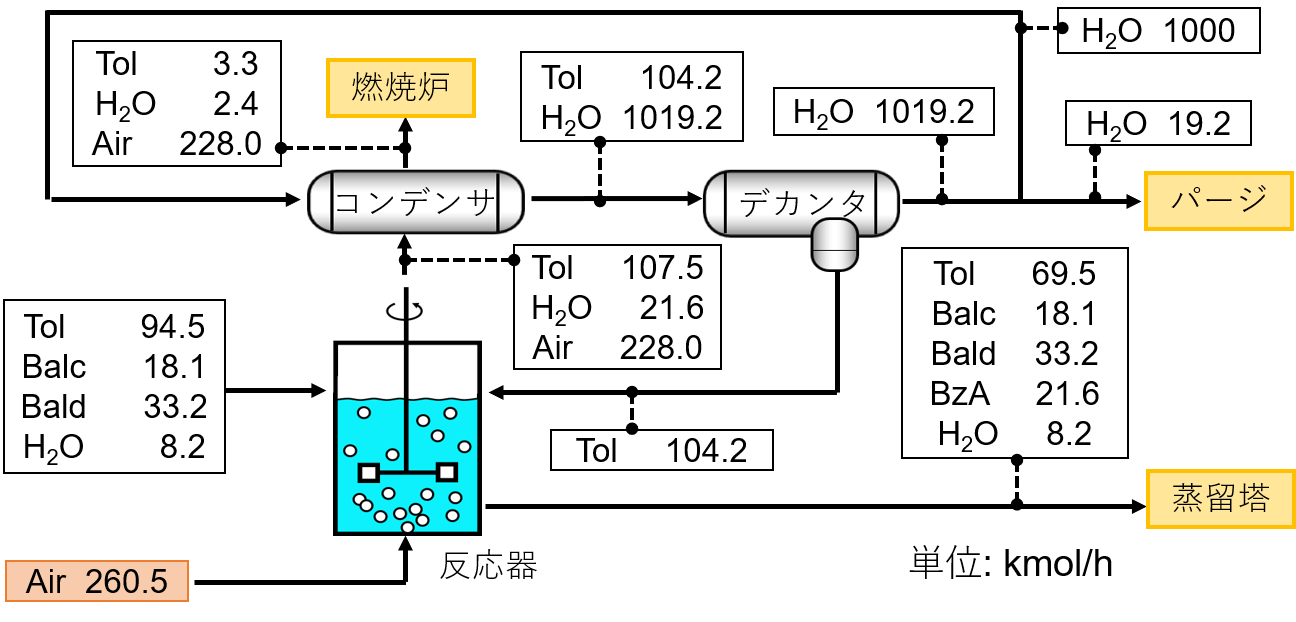
\includegraphics[scale=0.7]{ReactionSectionConclusion.png}
        \caption{反応部設計結果}
    \end{center}
\end{figure}


\newpage
\chapter{分離部1}
\section{蒸留塔設計}
未反応トルエンのうち99\%以上を回収することを目的とした。
設計条件として、蒸留塔段数を10段、蒸留塔供給段は6段、還流比を1.0とした。

蒸留塔圧力を変更し、全体の利益を最大とする点について探索を行った。
反応器流出液圧力が7barであるため、最適な圧力であることが予想される。
蒸留塔の圧力を変化させ、人件費を除く全体の利益を評価関数としてプロットした
図\ref{蒸留塔圧力最適化}から、確かに7barで全体の利益が最大化されることを確認した。
\begin{figure}[h]
    \label{蒸留塔圧力最適化}
    \begin{center}
        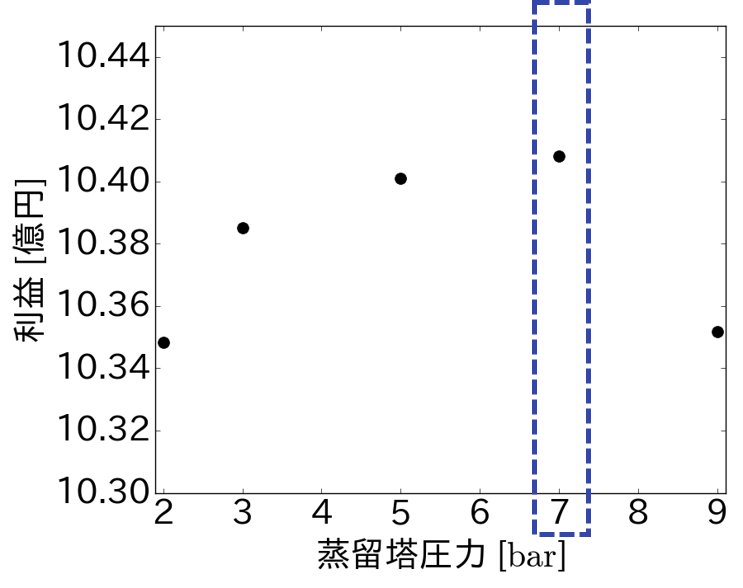
\includegraphics[scale=0.7]{DistillationPressue.png}
        \caption{蒸留塔圧力最適化}
    \end{center}
\end{figure}

設計結果を表\ref{蒸留塔設計結果}に記す。
\begin{table}[h]
    \label{蒸留塔設計結果}
    \caption{蒸留塔設計結果}
    \begin{center}
        \begin{tabular}{lc}\hline
            \multicolumn{1}{c}{項目}       &  値    \\   \hline
            塔径\,[m]                      &1.0    \\
            塔高\,[m]                      &6.1    \\
            塔内圧力\,[bar]                &7   \\
            コンデンサ内温度\,[\,$^\circ$C\,]       &232     \\
            リボイラー内温度\,[\,$^\circ$C\,]       &316    \\\hline
        \end{tabular}
    \end{center}
\end{table}

\section{分離部1設計結果}
最適化後の最終結果における分離部1の流量関係を図\ref{分離部1設計結果の図}中に示す。
\begin{figure}[h]
    \label{分離部1設計結果の図}
    \begin{center}
        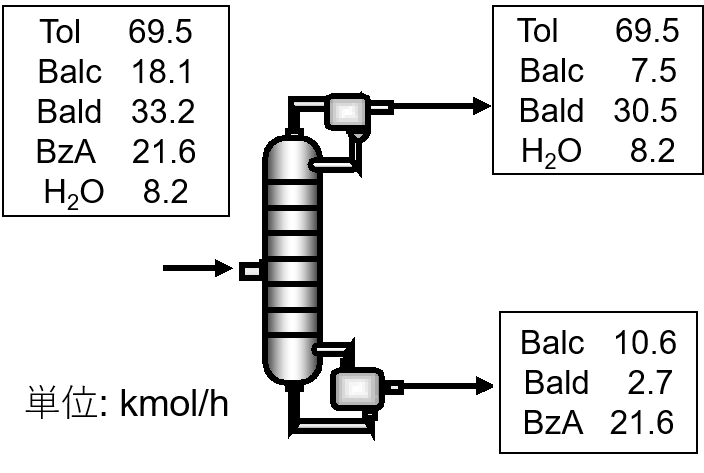
\includegraphics[scale=0.7]{Separation1Conclusion.png}
        \caption{分離部1設計結果}
    \end{center}
\end{figure}


\newpage
\chapter{分離部2}

\section{晶析器選定}
溶解度の温度依存性が大きいことと、目的とする結晶生産量が大きいことから、
連続式攪拌槽型反応装置を選定した。\\
溶解度の温度依存性の相関式
\begin{equation}
    C^*=2.03\times 10^{-5}T^4 +2.03^{-5}\times T^4 + 2.97\times 10^{-4}T^3 + 4.70\times 10^{-2}T^2
        + 1.43T + 24.71
\end{equation}
ただし,温度\,$T[\mathrm{^\circ C}]$,$C^*[\mathrm{g/kg-solvent}]$\\
\begin{figure}[h]
    \label{溶解度の温度依存性}
    \begin{center}
        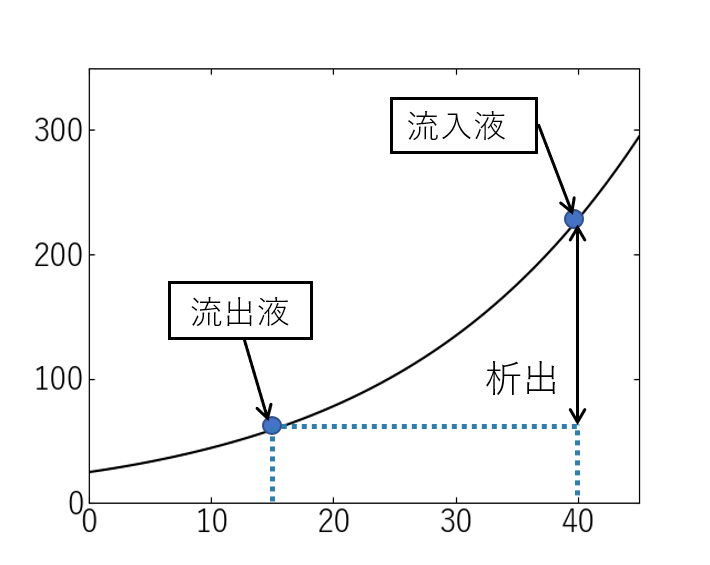
\includegraphics[scale=0.7]{BzAsolvent.png}
        \caption{溶解度の温度依存性}
    \end{center}
\end{figure}


\section{設計方程式}
以下の仮定を用いた。
\begin{itemize}
    \setlength{\parskip}{0pt}
    \setlength{\itemsep}{2pt} 
    \item[-] 結晶表面拡散は迅速に行われる。
    \item[-] 晶析器内は完全混合状態である。
    \item[-] 二次核発生の影響は無視する。
\end{itemize}

参考文献\cite{晶析}により、以下の実験式および理論式を用いて設計を行った。\\
一次核発生速度
\begin{equation}
    B^0 = k_{\mathrm{ b}}M_{\mathrm{ T}}^j \Delta C^b
\end{equation}
結晶成長速度
\begin{equation}
    G = k_{\mathrm{ g}}\Delta C^g
\end{equation}
結晶成長速度定数
\begin{equation}
    k_{\mathrm{ g}} = k_{\mathrm{ g0}} \exp(-\frac{E_{\mathrm{ g}}}{RT})
\end{equation}
個数収支式
\begin{equation}
    n=n^0 \exp(-\frac{L}{G\tau})
\end{equation}
懸濁密度
\begin{equation}
    M_{\mathrm{ T}} = c_0-c = 6k_{\mathrm{ v}}\rho_{\mathrm{ c}}n^0(G\tau)^4
\end{equation}
各パラメータは以下の通りである。
\begin{itemize}
    \item[] $k_{\mathrm{ g0}}\,=\,1.06\times10^7\,\mathrm{ (\mu m)/(g/g-solvent)^g}$
    \item[] $B^{\mathrm{ 0}}\,=\,40.05\,\mathrm{ kJ/mol}$
    \item[] $k_{\mathrm{ b}}\,=\,9.16\times10^12\,\mathrm{ (\#/ m^3\,s)/\{(g/mL)^{{\it j}}(g/g-solvent)^{{\it b}}\}}$
    \item[] $g\,=\,0.44\,$
    \item[] $j\,=\,1.78\,$
    \item[] $b\,=\,1.2\,$
    \item[] $k_{\mathrm{ v}}\,=\,0.1\,$
    \item[] $\rho_{\mathrm{ c}}\,=\,1.32\,\mathrm{ g/cm^3}$ 
\end{itemize}

\section{晶析器設計結果}
最適化の結果によって得られた晶析器の設計結果を以下に記す。

\section{抽出塔設計}
十分に塔内へ液を滞留させることによって安息香酸を水中に飽和させることを目的とした。
十分なデータを得られなかったため、2時間の装置内滞留によって安息香酸がトルエン溶媒中に飽和し、
その他ベンジルアルコール、ベンズアルデヒドの溶解度については無視できると仮定した。

\section{分離部2設計結果}
\begin{figure}[h]
    \label{分離部2設計結果}
    \begin{center}
        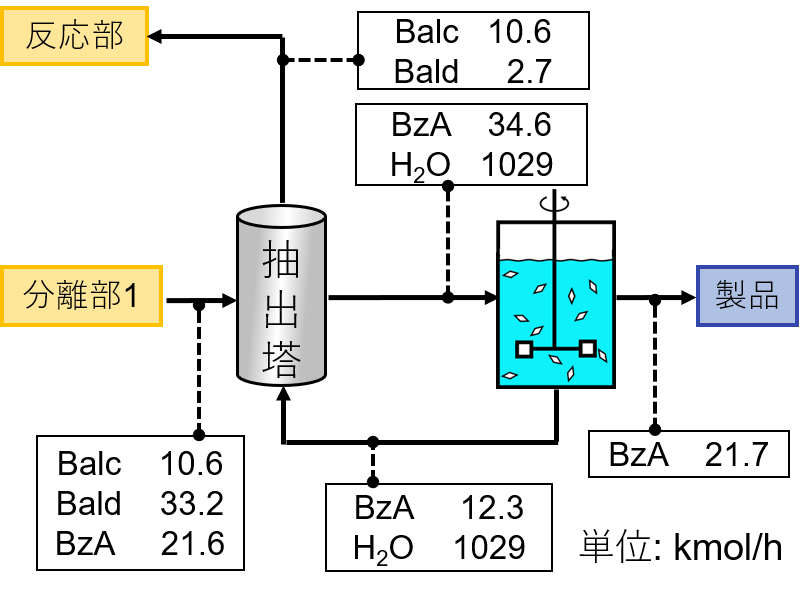
\includegraphics[scale=0.7]{Separion2Conclusion.png}
        \caption{分離部2設計結果}
    \end{center}
\end{figure}

\newpage
\chapter{最適化}
\section{方法}

\section{蒸留塔圧力の最適化}

\section{晶析器内温度の最適化}

\newpage
\chapter{物質収支 $\cdot$ 熱収支}
全体のフロー図および流量関係は下図のようになった。

全体の熱量関係は以下のようになった。

\newpage
\chapter{ヒートインテグレーション}
流体同士の熱交換を行い、外部流体の利用量を削減した。
図\ref{TQ線図}に最終的な設計結果におけるTQ線図を示す。
\begin{figure}[h]
    \label{TQ線図}
    \begin{center}
        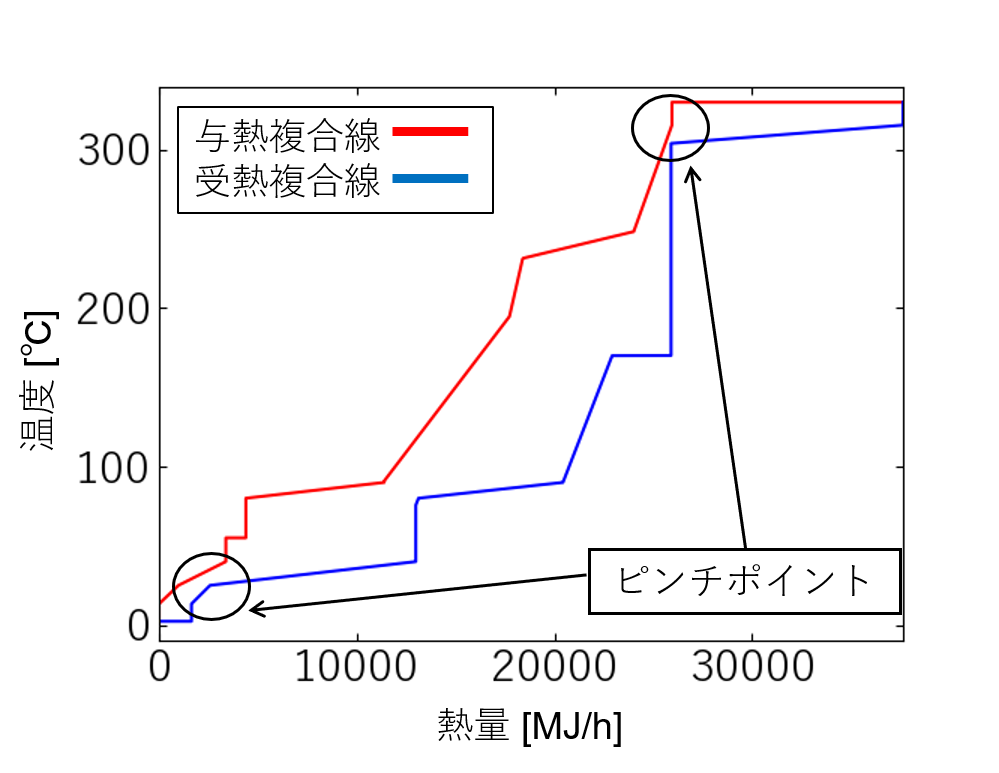
\includegraphics[scale=0.7]{TQdiagram.png}
        \caption{TQ線図}
    \end{center}
\end{figure}

熱交換により、外部熱媒を用いた場合と比較して、

\newpage
\chapter{経済評価}

\newpage
\chapter{結言}
設計目標を純度99.0wt\%の安息香酸を年2万ton製造するものとして、設計を行った。
文献値を参考として気液反応器、および晶析装置を設計した。
リサイクルフローを考えて、物質の有効利用を行った。
反応器体積、晶析器体積、晶析器内温度を用いたプロセス全体の3変数同時最適化を行った。
これにより、年 億円の利益を得ると見込める設計となった。\\
残った課題としては、蒸発トルエンのさらなる回収を行うため、燃焼炉ではなく吸着装置を用いることを検討することや、
各装置についてさらに詳細に設計することが挙げられる。

\newpage
\chapter*{謝辞}
\addcontentsline{toc}{chapter}{謝辞}
今回のプロセス設計では、様々な方々にお世話になりました。山本教授、谷口准教授を
はじめとする多くの化学工学の先生方、集中講義を実施してくださった玉川先生に感謝の意を申し上げます。\\
また、1講座の先輩方の協力無しには私たちのプロセス設計は実現できませんでした。
プロセスの内容や発表に対し、的確なアドバイスをいただきました。
お忙しい中、原稿やスライドのチェック、発表練習などに協力して頂いたことで、無事に発表を終えることができました。\\
私たちのプロセス設計に協力してくださった先生方、先輩方に改めて御礼申し上げます。

\newpage
\begin{thebibliography}{10}
    \bibitem{化工便覧} 化学工学便覧・化学工学会・丸善出版
    \bibitem{晶析} Gary Morris and  Graham Power {\it et al.  Org. Process Res. Dev.} {\bf 19}, 1891-1902, 2015
    \bibitem{キー} 参考文献の名前・著者N
\end{thebibliography}

\newpage
\chapter*{変数一覧}
\addcontentsline{toc}{chapter}{変数一覧}
\begin{multicols}{2}
\begin{flushleft}
$
    a:\text{比界面積} \\
    B^0:\text{一次核発生速度}\\
    c:\text{重量濃度}\\
    C:\text{モル濃度}\\
    C_{\mathrm{D}}:\text{抗力係数}\\
    D:\text{拡散係数}\\
    d_{\mathrm{vs}}:\text{気泡体積平均径}\\
    E:\text{活性化エネルギー}\\
    E_{\mathrm{g}}:\text{結晶化過程の活性化エネルギー}\\
    F:\text{モル流量}\\
    g:\text{重力加速度}\\
    G:\text{核成長速度}\\
    k:\text{反応速度定数}\\
    k_{\mathrm{b}}:\text{核発生速度定数}\\
    k_{\mathrm{g}}:\text{核成長速度定数}\\
    k_{\mathrm{L}}:\text{液相物質移動係数}\\
    k_{\mathrm{L}}a:\text{液相物質移動容量係数}\\
    k_{\mathrm{v}}:\text{結晶体積形状係数}\\
    M_{\mathrm{T}}:\text{懸濁密度}\\
    n:\text{結晶の個数密度}\\
    P_{\mathrm{G}}:\text{攪拌動力}\\
    P_{\mathrm{T}}:\text{}\\
    r:\text{反応速度定数}\\
    T:\text{温度}\\
    T_{\mathrm{c}}:\text{臨界温度}\\
    u_{\mathrm{t}}:\text{気泡の終末速度}\\
    u_{\mathrm{G}}:\text{気泡の空塔速度}\\
    V:\text{体積}\\
    \beta:\text{還流率}\\
    \mu:\text{粘度}\\
    \mu_{\mathrm{L}}:\text{液相粘度}\\
    \sigma:\text{界面張力}\\
    \rho_{\mathrm{a}}:\text{空気密度}\\
    \rho_{\mathrm{L}}:\text{液相密度}\\
    \rho_{\mathrm{g}}:\text{気相密度}\\
    \Delta\rho:\text{密度差}\\
    Eo:\text{エトベス数}\\
    Sc:\text{シュミット数}\\
    Re:\text{レイノルズ数}
$
\end{flushleft}
\end{multicols}


\chapter*{Appendix}
\addcontentsline{toc}{chapter}{Appendix}

\end{document}